\documentclass[tikz,border=10pt]{standalone}
\usepackage[T1]{fontenc}
\usepackage{tikz}
\usetikzlibrary{positioning,arrows.meta,fit,backgrounds,calc,shapes.geometric}

\definecolor{bgdark}{HTML}{1a1a1a}
\definecolor{fglight}{HTML}{e5e5e5}
\definecolor{accent}{HTML}{60a5fa}
\definecolor{muted}{HTML}{999999}
\definecolor{compilecolor}{HTML}{34d399}
\definecolor{linkcolor}{HTML}{fbbf24}
\definecolor{composecolor}{HTML}{f472b6}
\definecolor{boxbg}{HTML}{2a2a2a}

\begin{document}
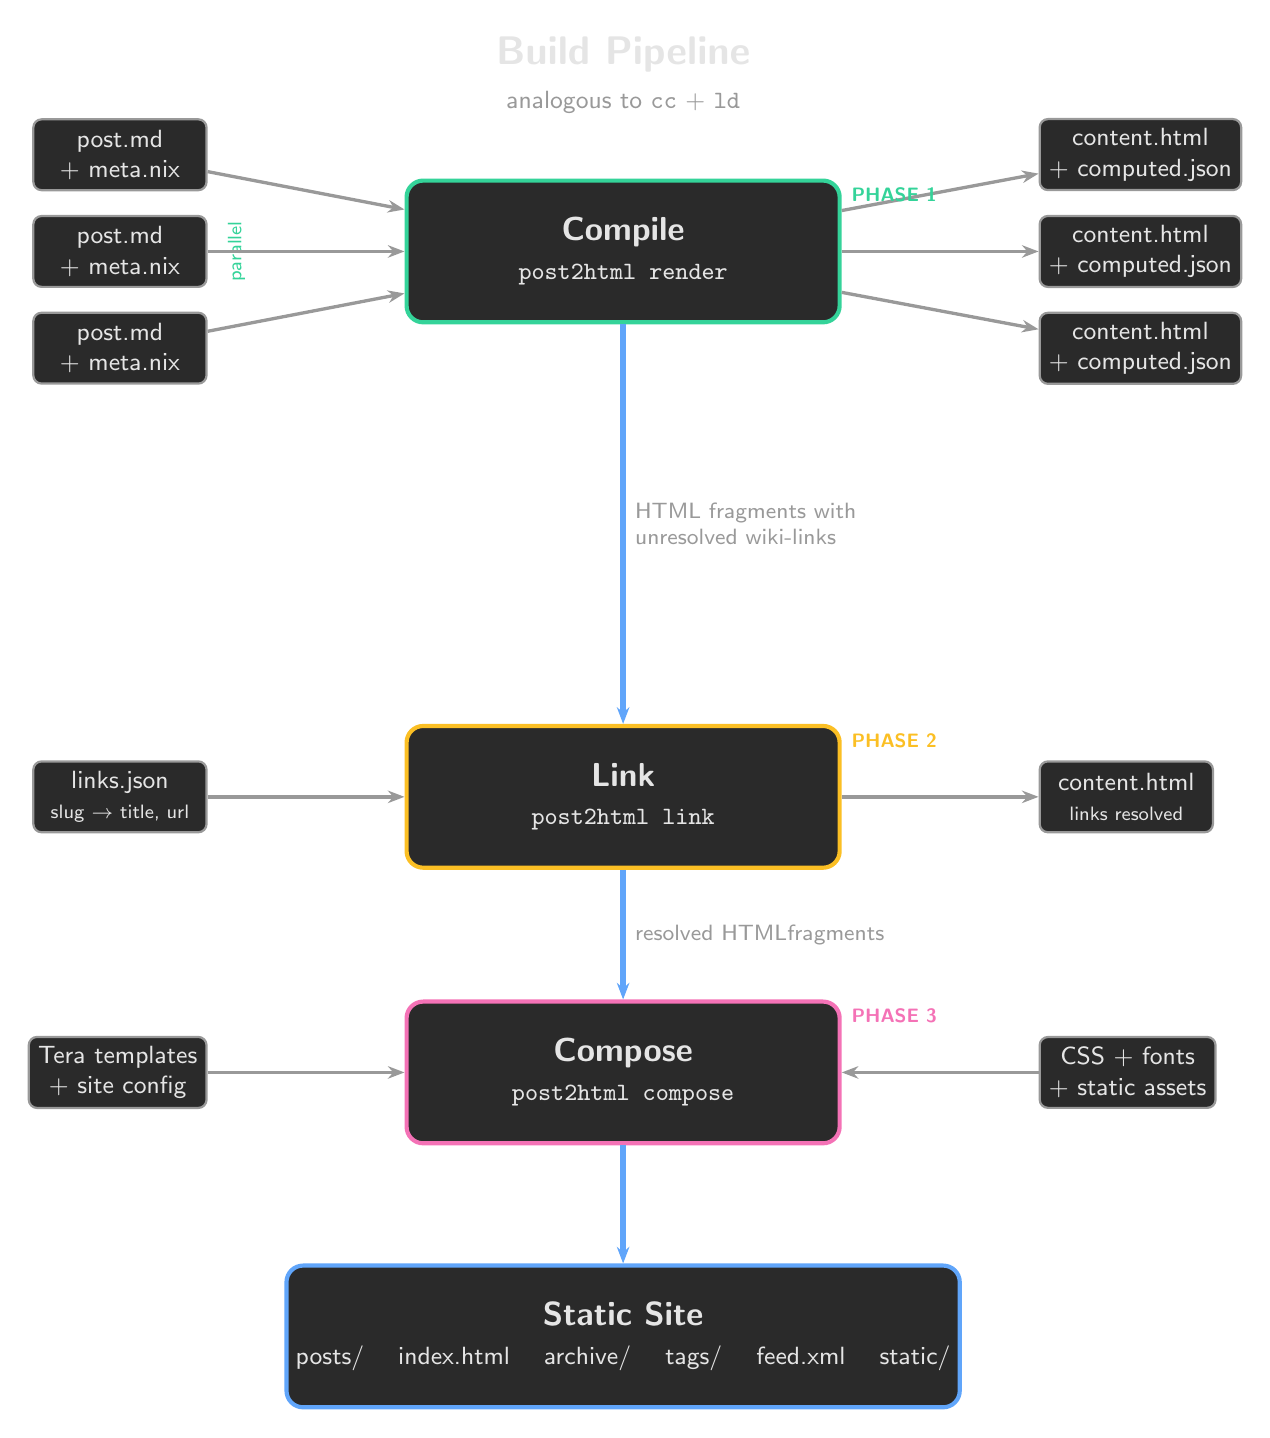
\begin{tikzpicture}[
    >={Stealth[length=6pt]},
    node distance=1.2cm and 1.8cm,
    every node/.style={font=\sffamily},
    phase/.style={
        rounded corners=6pt,
        minimum width=5.5cm,
        minimum height=1.8cm,
        align=center,
        text=fglight,
        draw=#1,
        line width=1.5pt,
        fill=boxbg,
    },
    smallbox/.style={
        rounded corners=3pt,
        minimum width=2.2cm,
        minimum height=0.9cm,
        align=center,
        text=fglight,
        draw=muted,
        line width=0.8pt,
        fill=boxbg,
        font=\sffamily\small,
    },
    input/.style={
        rounded corners=3pt,
        minimum width=2cm,
        minimum height=0.7cm,
        align=center,
        text=muted,
        font=\sffamily\scriptsize,
    },
    arrow/.style={->,line width=1.2pt,color=muted},
    phasearrow/.style={->,line width=2pt,color=accent},
    label/.style={font=\sffamily\footnotesize,text=muted},
]

% Title
\node[font=\sffamily\Large\bfseries,text=fglight] (title) at (0,6.5) {Build Pipeline};
\node[font=\sffamily\small,text=muted] at (0,5.9) {analogous to \texttt{cc} + \texttt{ld}};

% Phase 1: Compile
\node[phase=compilecolor] (compile) at (0,4) {
    \textbf{\large Compile}\\[2pt]
    {\small\texttt{post2html render}}
};
\node[label,anchor=east] at (compile.west) {};

% Parallel posts
\node[smallbox,left=2.5cm of compile] (post1) {post.md\\+ meta.nix};
\node[smallbox,above=0.3cm of post1] (post2) {post.md\\+ meta.nix};
\node[smallbox,below=0.3cm of post1] (post3) {post.md\\+ meta.nix};

% Compile outputs
\node[smallbox,right=2.5cm of compile] (frag1) {content.html\\+ computed.json};
\node[smallbox,above=0.3cm of frag1] (frag2) {content.html\\+ computed.json};
\node[smallbox,below=0.3cm of frag1] (frag3) {content.html\\+ computed.json};

% Parallel label
\node[font=\sffamily\scriptsize,text=compilecolor,rotate=90,anchor=south] at ($(post1.east)+(0.6,0)$) {parallel};

\draw[arrow] (post1) -- (compile);
\draw[arrow] (post2) -- (compile);
\draw[arrow] (post3) -- (compile);
\draw[arrow] (compile) -- (frag1);
\draw[arrow] (compile) -- (frag2);
\draw[arrow] (compile) -- (frag3);

% Phase 2: Link
\node[phase=linkcolor,below=2.5cm of compile] (link) at (0,0.5) {
    \textbf{\large Link}\\[2pt]
    {\small\texttt{post2html link}}
};

% Link input
\node[smallbox,left=2.5cm of link] (registry) {links.json\\{\scriptsize slug $\to$ title, url}};

\draw[phasearrow] (compile) -- node[right,label,align=left] {HTML fragments with\\unresolved wiki-links} (link);
\draw[arrow] (registry) -- (link);

% Link output
\node[smallbox,right=2.5cm of link] (resolved) {content.html\\{\scriptsize links resolved}};
\draw[arrow] (link) -- (resolved);

% Phase 3: Compose
\node[phase=composecolor,below=2.5cm of link] (compose) at (0,-3) {
    \textbf{\large Compose}\\[2pt]
    {\small\texttt{post2html compose}}
};

% Compose inputs
\node[smallbox,left=2.5cm of compose] (templates) {Tera templates\\+ site config};
\node[smallbox,right=2.5cm of compose] (theme) {CSS + fonts\\+ static assets};

\draw[phasearrow] (link) -- node[right,label] {resolved HTML\\fragments} (compose);
\draw[arrow] (templates) -- (compose);
\draw[arrow] (theme) -- (compose);

% Final output
\node[phase=accent,below=1.5cm of compose,minimum width=8cm] (output) {
    \textbf{\large Static Site}\\[2pt]
    {\small posts/ \quad index.html \quad archive/ \quad tags/ \quad feed.xml \quad static/}
};

\draw[phasearrow] (compose) -- (output);

% Phase labels — anchored to phase box right edge, below output boxes
\node[font=\sffamily\scriptsize\bfseries,text=compilecolor,anchor=north west] at (compile.north east) {PHASE 1};
\node[font=\sffamily\scriptsize\bfseries,text=linkcolor,anchor=north west] at (link.north east) {PHASE 2};
\node[font=\sffamily\scriptsize\bfseries,text=composecolor,anchor=north west] at (compose.north east) {PHASE 3};

\end{tikzpicture}
\end{document}
